\documentclass[crop,tikz]{standalone}
\usepackage{tikz}
\usepackage{ifthen}
\usepackage[scaled]{helvet}
\renewcommand*\familydefault{\sfdefault}

\begin{document}

\definecolor{yellow}{rgb}{1.0, 1.0, 0.45} % 255/255/115
\definecolor{dkyellow}{rgb}{0.9, 0.9, 0.0} % % 230/230/0

\definecolor{ltorange}{rgb}{1.0, 0.74, 0.41} % 255/188/105
\definecolor{orange}{rgb}{0.96, 0.50, 0.0} % 246/127/0

\definecolor{ltred}{rgb}{1.0, 0.25, 0.25} % 255/64/64
\definecolor{red}{rgb}{0.79, 0.00, 0.01} % 201/0/3

\definecolor{ltblue}{rgb}{0.2, 0.73, 1.0} % 51/187/255
\definecolor{blue}{rgb}{0.12, 0.43, 0.59} % 30/110/150

\definecolor{ltltgreen}{rgb}{0.7, 1.00, 0.7} % 96/204/14
\definecolor{ltgreen}{rgb}{0.37, 0.80, 0.05} % 96/204/14
\definecolor{green}{rgb}{0.23, 0.49, 0.03} % 59/125/8
  
\definecolor{dkslate}{rgb}{0.18, 0.21, 0.28} % 47/53/72
\definecolor{mdslate}{rgb}{0.45, 0.50, 0.68} % 114/127/173
\definecolor{ltslate}{rgb}{0.85, 0.88, 0.95} % 216/225/229

\usetikzlibrary{positioning,arrows.meta,shapes,calc,patterns}

% Basic entities
\tikzstyle{arrow} = [-{Latex[length=9pt,width=6pt]}]
\tikzstyle{rarrow} = [{Latex[length=9pt,width=6pt]}-]
\tikzstyle{vertex}=[circle,inner sep=1.5pt, minimum size=2mm]

\tikzstyle{bc}=[color=purple, line width=2.0pt]
\tikzstyle{bc-label}=[text=purple]

\tikzstyle{gdomain}=[fill=ltblue!25!white]

% Finite-element entities
\tikzstyle{point-label}=[]
\tikzstyle{fevertex}=[vertex, color=orange,fill=orange]
\tikzstyle{fevertex-label}=[point-label, text=orange]

\tikzstyle{cell}=[color=blue,line width=1.0pt]
\tikzstyle{cell-label}=[point-label, text=blue]


% Geometry entities
\tikzstyle{gvertex}=[vertex, color=orange,fill=orange]
\tikzstyle{gvertex-label}=[point-label, text=orange]

\tikzstyle{curve}=[line width=1.0pt, color=blue]
\tikzstyle{curve-dir}=[line width=1.0pt, arrow=>latex, color=blue]
\tikzstyle{curve-label}=[point-label, text=blue]


% Annotation
\tikzstyle{axes}=[line width=1.0pt, color=gray]
\tikzstyle{axes-label}=[font=\bfseries, color=gray]


\tikzstyle{roller}=[color=green,line width=1.0pt]
\tikzstyle{ground}=[fill,pattern color=green,pattern=north east lines,draw=none,anchor=north,minimum width=0.8cm,minimum height=0.3cm]


\tikzstyle{local-image} = [anchor=south west,inner sep=0]

\def\radius{0.025}%

\foreach \figpart in {1,...,5}{

% -------------------------------------------------------------------------------------------------
\begin{tikzpicture}

\ifthenelse{\figpart=2}{%
    \node[local-image] (image) at (0,0) {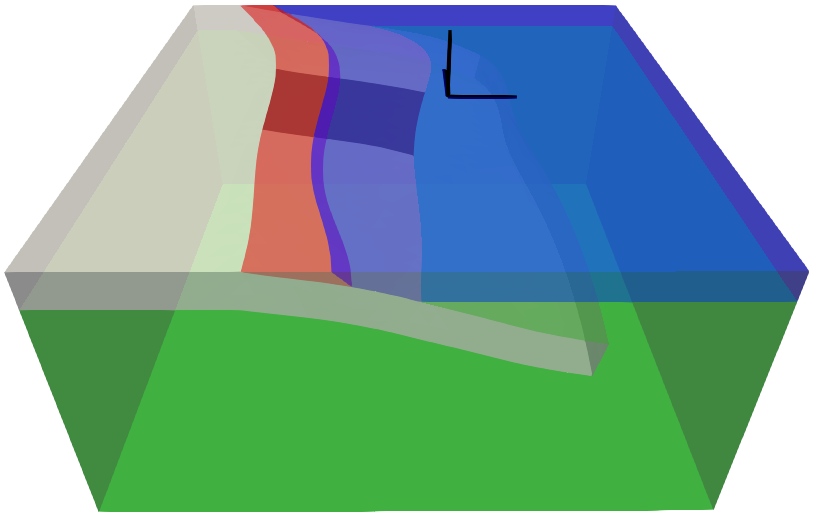
\includegraphics[width=5.5in]{cubit-geometry-patch.png}};
}{%
\ifthenelse{\figpart=5}{%
    \node[local-image] (image) at (0,0) {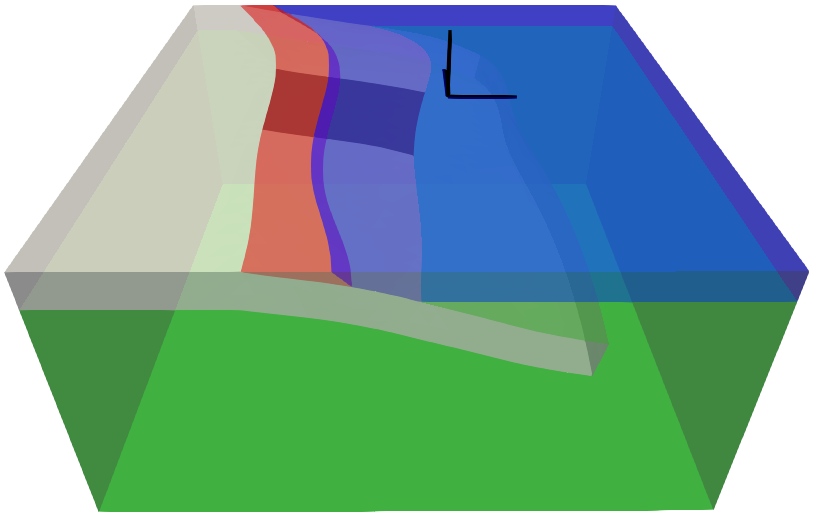
\includegraphics[width=5.5in]{cubit-geometry-patch.png}};
}{%
    \node[local-image] (image) at (0,0) {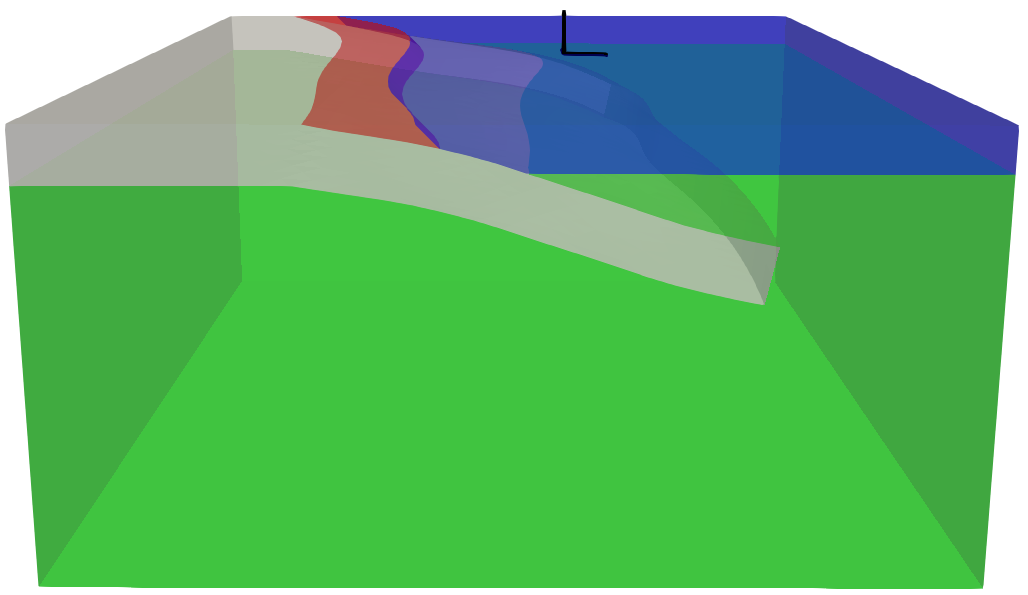
\includegraphics[width=5.5in]{cubit-geometry}};
}
}{}


% -------------------------------------------------------------------------------------------------
% Step 1 (axialdisp)
% -------------------------------------------------------------------------------------------------
\ifthenelse{\figpart=1}{
    \def\rspacing{0.25}%

    \begin{scope}[x={(image.south east)},y={(image.north west)}]
        % -x
        \node[anchor=west, bc-label] (xneg) at (-0.15,0.6) {+2.0 m};
        \draw[bc,arrow] (xneg) -- (0.15,0.6);

        % +x
        \node[anchor=east, bc-label] (xpos) at (+1.15,0.6) {-2.0 m};
        \draw[bc,arrow] (xpos) -- (0.85,0.6);

        % -z
        \foreach \ix in {0,...,3}{%
        \draw[roller] ($(0,0)+(\ix*\rspacing+0.5*\rspacing,-\radius)$) circle (\radius);
        \node[ground] at ($(0,0)+(\ix*\rspacing+0.5*\rspacing,-2*\radius)$) {};
        }
        \node[bc-label] at ($(0,0)+(0.5,-5*\radius)$) {$u_z=0$};

    \end{scope}

}{} % if/else


% -------------------------------------------------------------------------------------------------
% Step 2 (coseismic)
% -------------------------------------------------------------------------------------------------
\ifthenelse{\figpart=2}{
    \def\rspacing{0.285}%

\begin{scope}[x={(image.south east)},y={(image.north west)}]

    % Fault
    \node[anchor=west, bc-label] (xneg) at (0.12,0.70) {Uniform slip};
    \draw[bc,arrow] (xneg) -- (0.35,0.77);

    % -x
    \foreach \iy in {0,...,1}{%
    \draw[roller] ($(0.1,0)+(-\radius-\iy*0.07,\iy*\rspacing+0.2*\rspacing)$) circle (\radius);
    \node[ground, anchor=north, rotate=-90] at ($(0.1,0)+(-2*\radius-\iy*0.07,\iy*\rspacing+0.2*\rspacing)$) {};
    }
    \node[bc-label] at ($(0.1,0)+(-0.15,0.2)$) {$u_x=0$};

    % +x
    \foreach \iy in {0,...,1}{%
    \draw[roller] ($(0.9,0)+(+\radius+\iy*0.07,\iy*\rspacing+0.2*\rspacing)$) circle (\radius);
    \node[ground, anchor=north, rotate=+90] at ($(0.9,0)+(+2*\radius+\iy*0.07,\iy*\rspacing+0.2*\rspacing)$) {};
    }
    \node[bc-label] at ($(0.9,0)+(0.15,0.2)$) {$u_x=0$};

    % -z
    \foreach \ix in {0,...,2}{%
    \draw[roller] ($(0.1,0)+(\ix*\rspacing+0.4*\rspacing,-\radius)$) circle (\radius);
    \node[ground] at ($(0.1,0)+(\ix*\rspacing+0.4*\rspacing,-2*\radius)$) {};
    }
    \node[bc-label] at ($(0,0)+(0.5,-5*\radius)$) {$u_z=0$};

\end{scope}

}{} % if/else


% -------------------------------------------------------------------------------------------------
% Step 3 (interseismic)
% -------------------------------------------------------------------------------------------------
\ifthenelse{\figpart=3}{
    \def\rspacing{0.25}%

\begin{scope}[x={(image.south east)},y={(image.north west)}]

    % Bottom of slab, subduction interface (deep)
    \node[anchor=east, bc-label] (creep) at (0.50,0.45) {Creep};
    \draw[bc,arrow] (creep.north) -- (0.60,0.65);
    \draw[bc,arrow] (creep.north) -- (0.60,0.55);
    \draw[bc,arrow] (creep.north) -- (0.30,0.68);

    % Subduction interface: shallow
    \node[anchor=east, bc-label] (locked) at (0.30,0.72) {Locked};
    \draw[bc,arrow] (locked) -- (0.38,0.76);

    % Slab not include in BC
    \node[anchor=east, bc-label, text width=1.0in] (bcnote) at (0,0.90) {Exclude slab\\ from Dirichlet BCs};
    \draw[bc,arrow] (bcnote) -- (0.10,0.85);

    % -x
    \foreach \iy in {0,...,2}{%
    \draw[roller] ($(0.03,0)+(-\radius-\iy*0.01,\iy*\rspacing+0.5*\rspacing)$) circle (\radius);
    \node[ground, anchor=north, rotate=-90] at ($(0.03,0)+(-2*\radius-\iy*0.01,\iy*\rspacing+0.5*\rspacing)$) {};
    }
    \node[bc-label] at ($(0.03,0)+(-0.12,0.5)$) {$u_x=0$};

    % +x
    \foreach \iy in {0,...,2}{%
    \draw[roller] ($(0.97,0)+(+\radius+\iy*0.01,\iy*\rspacing+0.5*\rspacing)$) circle (\radius);
    \node[ground, anchor=north, rotate=+90] at ($(0.97,0)+(+2*\radius+\iy*0.01,\iy*\rspacing+0.5*\rspacing)$) {};
    }
    \node[bc-label] at ($(0.97,0)+(0.12,0.5)$) {$u_x=0$};

    % -z
    \foreach \ix in {0,...,3}{%
    \draw[roller] ($(0,0)+(\ix*\rspacing+0.5*\rspacing,-\radius)$) circle (\radius);
    \node[ground] at ($(0,0)+(\ix*\rspacing+0.5*\rspacing,-2*\radius)$) {};
    }
    \node[bc-label] at ($(0,0)+(0.5,-5*\radius)$) {$u_z=0$};

\end{scope}

}{} % if/else


% -------------------------------------------------------------------------------------------------
% Step 4 (eqcycle)
% -------------------------------------------------------------------------------------------------
\ifthenelse{\figpart=4}{
    \def\rspacing{0.25}%

\begin{scope}[x={(image.south east)},y={(image.north west)}]

    % Bottom of slab, subduction interface (deep)
    \node[anchor=east, bc-label] (creep) at (0.50,0.45) {Creep};
    \draw[bc,arrow] (creep.north) -- (0.60,0.65);
    \draw[bc,arrow] (creep.north) -- (0.60,0.55);
    \draw[bc,arrow] (creep.north) -- (0.30,0.68);

    % Subduction interface: shallow
    \node[anchor=east, bc-label] (eqs) at (0.35,0.72) {Earthquakes};
    \draw[bc,arrow] (eqs.east) -- (0.41,0.78);
    \draw[bc,arrow] (eqs.east) -- (0.45,0.74);

    % Slab not include in BC
    \node[anchor=east, bc-label, text width=1.0in] (bcnote) at (0,0.90) {Exclude slab\\ from Dirichlet BCs};
    \draw[bc,arrow] (bcnote) -- (0.10,0.85);

    % -x
    \foreach \iy in {0,...,2}{%
    \draw[roller] ($(0.03,0)+(-\radius-\iy*0.01,\iy*\rspacing+0.5*\rspacing)$) circle (\radius);
    \node[ground, anchor=north, rotate=-90] at ($(0.03,0)+(-2*\radius-\iy*0.01,\iy*\rspacing+0.5*\rspacing)$) {};
    }
    \node[bc-label] at ($(0.03,0)+(-0.12,0.5)$) {$u_x=0$};

    % +x
    \foreach \iy in {0,...,2}{%
    \draw[roller] ($(0.97,0)+(+\radius+\iy*0.01,\iy*\rspacing+0.5*\rspacing)$) circle (\radius);
    \node[ground, anchor=north, rotate=+90] at ($(0.97,0)+(+2*\radius+\iy*0.01,\iy*\rspacing+0.5*\rspacing)$) {};
    }
    \node[bc-label] at ($(0.97,0)+(0.12,0.5)$) {$u_x=0$};

    % -z
    \foreach \ix in {0,...,3}{%
    \draw[roller] ($(0,0)+(\ix*\rspacing+0.5*\rspacing,-\radius)$) circle (\radius);
    \node[ground] at ($(0,0)+(\ix*\rspacing+0.5*\rspacing,-2*\radius)$) {};
    }
    \node[bc-label] at ($(0,0)+(0.5,-5*\radius)$) {$u_z=0$};

\end{scope}

}{} % if/else


% -------------------------------------------------------------------------------------------------
% Step 6 (slowslip)
% -------------------------------------------------------------------------------------------------
\ifthenelse{\figpart=5}{
    \def\rspacing{0.285}%

\begin{scope}[x={(image.south east)},y={(image.north west)}]

    % Fault
    \node[anchor=west, bc-label] (xneg) at (0.12,0.70) {Prescribed slip};
    \draw[bc,arrow] (xneg) -- (0.35,0.77);
    
    % -x
    \foreach \iy in {0,...,1}{%
    \draw[roller] ($(0.1,0)+(-\radius-\iy*0.07,\iy*\rspacing+0.2*\rspacing)$) circle (\radius);
    \node[ground, anchor=north, rotate=-90] at ($(0.1,0)+(-2*\radius-\iy*0.07,\iy*\rspacing+0.2*\rspacing)$) {};
    }
    \node[bc-label] at ($(0.1,0)+(-0.15,0.2)$) {$u_x=0$};

    % +x
    \foreach \iy in {0,...,1}{%
    \draw[roller] ($(0.9,0)+(+\radius+\iy*0.07,\iy*\rspacing+0.2*\rspacing)$) circle (\radius);
    \node[ground, anchor=north, rotate=+90] at ($(0.9,0)+(+2*\radius+\iy*0.07,\iy*\rspacing+0.2*\rspacing)$) {};
    }
    \node[bc-label] at ($(0.9,0)+(0.15,0.2)$) {$u_x=0$};

    % -z
    \foreach \ix in {0,...,2}{%
    \draw[roller] ($(0.1,0)+(\ix*\rspacing+0.4*\rspacing,-\radius)$) circle (\radius);
    \node[ground] at ($(0.1,0)+(\ix*\rspacing+0.4*\rspacing,-2*\radius)$) {};
    }
    \node[bc-label] at ($(0,0)+(0.5,-5*\radius)$) {$u_z=0$};

\end{scope}

}{} % if/else


\end{tikzpicture}}
\end{document}
